\chapter{Kleine Motoren/Machines (Small Motors)}
Nu gaan we kijken naar een paar speciale types motoren, vooral toepassingen van de motoren
die we tot nu toe gezien hebben.
De verschillende motoren waarover we het gaan hebben zijn de volgende:

\begin{itemize}
    \item 1-fasige motoren (deze vind je vooral thuis in apparaten zoals wasmachines,
    stofzuigers, $\cdots$)
    \begin{itemize}
     \item Universeel motoren
     \item 1-fasige inductie motor (Gewone 1f inductiemotor, Condensator motor, Spleetpool
     motor)
    \end{itemize}
    \item Vermogen elektronica gestuurde motoren
    \begin{itemize}
        \item BLDC (vooral de deze is belangrijk)
        \item Reluctantie motoren
        \item Stepper motoren
    \end{itemize}
\end{itemize}

\section{Universeel motor}
Universeel motors zijn \textbf{DC-seriemotoren} die werken op zowel AC als DC (1-fasig),
dit is waarom we het zoveel in huishoudtoestellen vinden, het zijn eigelijk variaties van
een DC-machine.
Een motor die dus zowel op een batterij (DC) als op het stopcontact (AC) werkt.
Maar hoe werkt dit?
Daarvoor gaan we even terug naar de vergelijkingen voor een DC-machine:
\begin{align*}
 E = k \cdot \varphi \cdot \omega = G \cdot I_e \cdot \omega \\
 T = k \cdot \varphi \cdot I_a = G \cdot I_e \cdot I_a
\end{align*}

\begin{figure}[H]
  \centering
  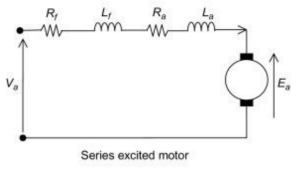
\includegraphics[width=0.5\textwidth]{assets/dcserieschakelele.png}
  \caption{Herhaling DC-serie schakeling}
  \label{fig:dcserieschakelele.png}
 \end{figure}

Uit de DC-serie schakeling weten we ook dat $I_e = I_a = I$, bij een shun bekrachtiging
worden deze stromen apart aangestuurd, als je dat dan op AC aansluit dan wisselt het
statorveld steeds van polariteit.
Als de ankerstroom daar niet perfect synchroon mee wissel, keert op sommige momenten of
het veld of de stroom van teken, nooit beide, en dan wordt het koppel
$T = G \cdot I_e \cdot I_a$ altijd negatief en het resulterende gemiddelde koppel over een
periode wordt zo goed als nul.
Conclusie:
bij een shunt bekrachtiging gaat AC de motor niet doen draaien, alleen een beetje trillen.
Bij een serie bekrachtiging is dit anders, want de stroom door de ankerwikkeling en de
veldwikkeling is dezelfde, dus als het veld van teken wisselt dan wisselt de ankerstroom
ook van teken en blijft het koppel $T = G \cdot I_e \cdot I_a$ altijd positief.
Het resulterende gemiddelde koppel over een periode is dus niet nul en de motor draait
gewoon verder.
Dit is dus waarom een DC-serie motor op AC kan werken.
Kan je ook zien aan het feit dat $T = G \cdot I^2$ een kwadraat heeft (altijd positief).

\begin{figure}[H]
  \centering
  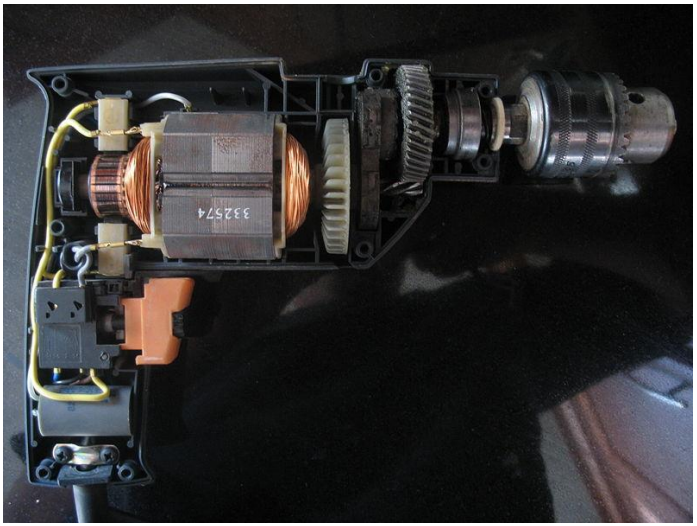
\includegraphics[width=0.5\textwidth]{assets/voorbeeldbooruniverseelmotor.png}
  \caption{Voorbeeld van een universele motor}
  \label{fig:voorbeeldbooruniverseelmotor.png}
 \end{figure}

In de figuur een voorbeeld van een universele motor in een boor, je kan hier duidelijk de
commutator zien.

Dit hebben we eigelijk al eerder gezien, maar hier wordt het rap herhaald maar als we de
inwendige spanning invullen in de spanningsvergelijking kunnen we omvormen naar de stroom
en dit invullen in de koppel formule om een vergelijking van het koppel toerental
karakteristiek te bekomen:
\begin{align*}
 U_a = E + R_a \cdot I = G \cdot I \cdot \omega + R_a \cdot I \\
\Rightarrow I = \frac{U_a}{G \cdot \omega + R_a} \\
\Rightarrow T = G \cdot I^2 = G \cdot \left(\frac{U_a}{G \cdot \omega + R_a}\right)^2
\end{align*}
Dit vormt dus de eerder geziene hyperbole T-n karakteristiek:

\begin{figure}[H]
  \centering
  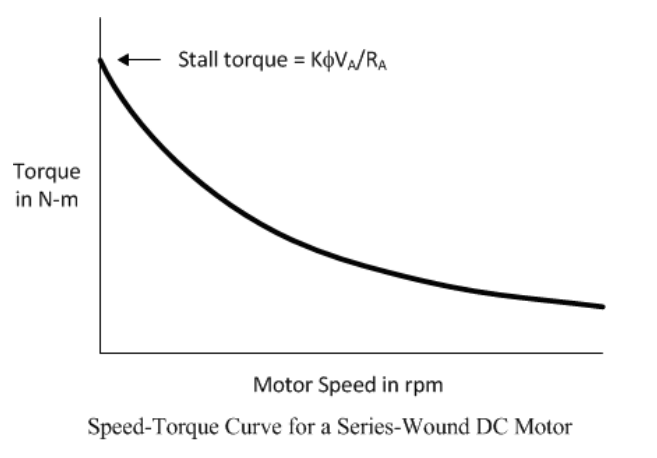
\includegraphics[width=0.5\textwidth]{assets/TNseriemootr.png}
  \caption{T-n karakteristiek van een DC-serie motor}
  \label{fig:TNseriemootr.png}
 \end{figure}

\subsection{Nadelen van een universele motor}
({\color{red}Deels door AI gecooked hier, maar het klopt allemaal})
\newline
En dan komen we nu ook terug op 1 van die grote nadelen dat al besproken was, namelijk dat
als je koppel naar 0 gaat, de snelheid naar oneindig gaat (wat we ook op onze
karakteristiek zien).
Wat het extra gevaarlijk hier maakt is het feit dat als de stroom daalt (dat trouwens ook
evenredig is aan het veld) dat het koppel hard daalt (kwadratisch) en dus ook het veld, en
om $E \approx V_\phi$ te houden moet de snelheid dan stijgen omdat ons veld zo zwak is.
Dit heet dus \textbf{'op hol slaan'} en is in theoretisch naar oneindig maar in het echt
zijn er verliezen enzo dus gaat dit gewoon heel hoog worden.

Een ander nadeel is dat als de motor stil staat dat er een heel grote stroom door de
wikkelingen gaat (want $E = 0$ dus $I = \frac{U}{R}$) en dit kan de wikkelingen doen
verbranden zeker als de rotor geblokkeerd is, bvb als je boor vast zit.
Meestal is er wel een soort van zekering voorzien.

Een volgend nadeel is dat het koppel \textbf{pulseert}.
Bij een zuivere DC-seriemotor is de stroom constant, dus is het koppel dat ook.
Bij de universele motor (op AC) is de stroom sinusvormig, en aangezien $T = G \cdot I^2$,
is het koppel dus een gekwadrateerde sinus, het blijft wel altijd positief (want een
kwadraat), maar het is niet meer vlak, het pulseert tussen 0 en een piekwaarde aan het
dubbele van de netfrequentie.
Dat geeft trillingen en geluid, en is meteen ook de reden waarom je een universele motor
bijna uitsluitend thuis tegenkomt (boormachine, mixer, stofzuiger) en niet in de
industrie, waar je meestal een vlakkere, trillingsvrije aandrijving wil.

\begin{figure}[H]
  \centering
  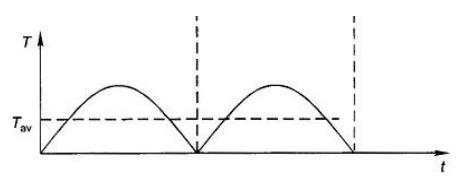
\includegraphics[width=0.6\textwidth]{assets/pulserendkoppel.png}
  \caption{Pulserend koppel van een universele motor op AC}
  \label{fig:pulserendkoppel.png}
 \end{figure}

Er zijn ook extra \textbf{ijzerverliezen} door de statorconstructie.
Bij een zuivere DC-motor is het statorveld constant, dus is er geen hysteresis- of
wervelstroomverlies in het statorijzer, en volstaat een massieve (niet-gelamelleerde)
statorkern.
Bij AC wisselt het statorveld wel voortdurend mee met de netfrequentie, wat in een
massieve kern net wel hysteresis- en wervelstroomverliezen zou geven.
Daarom moet de stator van een universele motor, net zoals de rotor, ook
\textbf{gelamelleerd} gebouwd worden, wat extra kost en complexiteit met zich meebrengt
die een zuivere DC-seriemotor niet heeft.
(De rotor is trouwens sowieso altijd gelamelleerd, ook bij DC, want vanuit een
rotorgeleider gezien wisselt het veld toch, aangezien die geleider om beurten een noord-
en een zuidpool voorbij ziet komen terwijl hij ronddraait.)

Een gerelateerd nadeel is de grotere invloed van de \textbf{terug-emk (back-emf)}.
De volledige spanningsvergelijking is:
\begin{align*}
 U_a = E + R_a I_a + L_a \frac{di_a}{dt}.
\end{align*}
Bij DC in stationair regime is $\frac{di_a}{dt}=0$, dus die term valt weg.
Bij AC verandert de stroom voortdurend, dus dat spanningsvalletje over de inductantie is
er altijd bij en 'eet' een deel van $U_a$ op.
Er blijft dan minder spanning over voor $E$, en aangezien
$E = C\varphi\omega = G \cdot I \cdot \omega$, betekent minder $E$ bij dezelfde stroom een
lagere snelheid voor dezelfde effectieve voedingsspanning.
De universele (AC-)versie draait dus trager dan de zuivere DC-versie bij gelijke spanning
en belasting.

Dit wordt ook mooi bevestigd op de koppel-snelheidsgrafiek:
bij eenzelfde percentage van het vollastkoppel ligt de snelheidscurve voor DC-voeding
hoger dan die voor AC-voeding.
Met andere woorden:
dezelfde motor presteert altijd net iets beter op DC dan op AC, precies door de extra
ijzer- en inductieverliezen hierboven.

Een laatste ding dat we ook nog kunnen zien in volgende figuur is dat we een iets lager
koppel hebben als we de universele motor op AC aansluiten:

\begin{figure}[H]
  \centering
  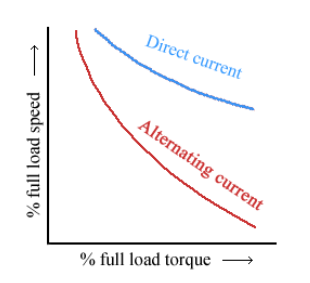
\includegraphics[width=0.4\textwidth]{assets/ACDCTN.png}
  \caption{AC vs DC T-n karakteristiek van een universele motor}
  \label{fig:ACDCTN.png}
 \end{figure}

\section{1-fasige inductie motor}
Dan kijken we nu naar de andere éénfasige motor, de 1-fasige inductie motor.
Net zoals de universele motor mag deze motor op het stopcontact.
Voor opbouw berschilt deze niet te veel van de normale inductiemotor, hij heeft ook een
\textbf{kooirotor} die eigelijk exact hetzelfde is.
Het is bij de stator dat er wat verschil is want hier hebben we namelijk \textbf{1
statorwikkeling} (want we kunnen maar 1 fase aansluiten).
Ook heeft deze motor een \textbf{centrifugaal schakelaar}, dit is een mechanische
schakelaar die reageert op de rotatiesnelheid, hij schakelt om zodra de rotor een bepaalde
snelheid bereikt (Het nut hiervan zien we zometeen).

\begin{figure}[H]
  \centering
  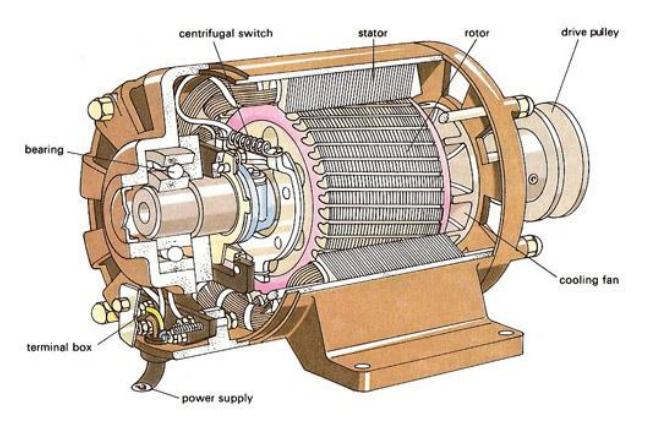
\includegraphics[width=0.5\textwidth]{assets/eenfasigeinductiemachine.png}
  \caption{Eénfasige inductiemachine}
  \label{fig:eenfasigeinductiemachine.png}
 \end{figure}

De koppel-toerental karakteristiek van deze motor ziet er als volgt uit (het is die
Single-phase op de figuur):

\begin{figure}[H]
  \centering
  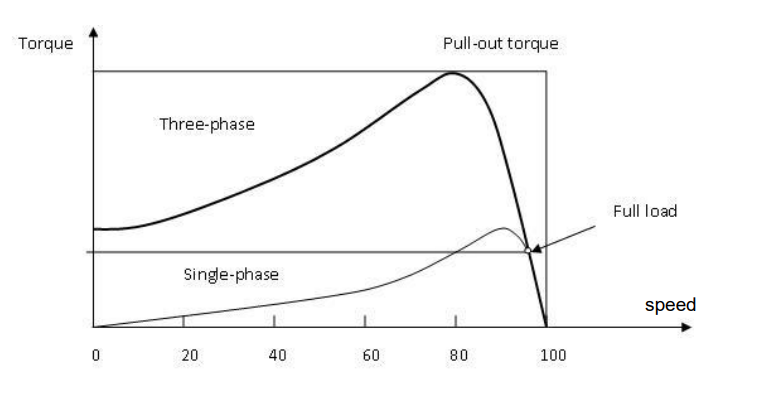
\includegraphics[width=0.6\textwidth]{assets/TNeenfasigeim.png}
  \caption{Koppel-toerental karakteristiek van een éénfasige inductiemachine}
  \label{fig:TNeenfasigeim.png}
 \end{figure}

Hier op zien we een probleem, namelijk dat bij de 1-fasige inductiemachine er \textbf{geen
startkoppel} is, dit omdat een stator met maar 1 wikkeling enkel een wisselveld geeft, er
is geen draaiveld.
Dit wisselveld induceert wel spanning/stroom in de rotorstaven maar zoals de grafiek toont
is het koppel 0 op n = 0 dus kan het niet starten.
De motor heeft dus wel een soort synchrone snelheid waarbij het koppel nul wordt zoals bij
de normale inductiemotor.
\textit{Van zodra de 1-fasige inductiemotor draait levert hij wel koppel.}

\subsection{Werking van de 1-fasige inductiemachine}
Hoezo heeft een wisselveld nog koppel eigelijk?
We gaan het als volgt bekijken, we hebben in de volgende figuur ons wissledveld, dit kan
beschreven worden als een staande golf (hier in het zwart).
Ook kan dit puur pulserend veld beschreven worden als de som van \textbf{twee even grote
velden die met dezelfde snelheid in tegengestelde richting ronddraaien}.
Op de figuur is dit de paarse curve (een som van een blauwe en rode curve in tegengestelde
richting):

\begin{figure}[H]
  \centering
  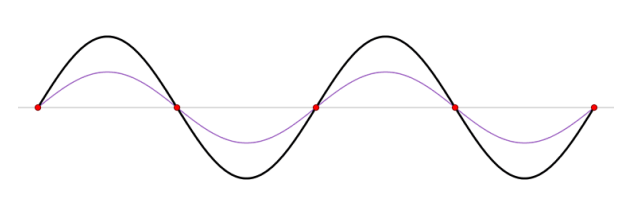
\includegraphics[width=0.8\textwidth]{assets/veld1fasigeIM.png}
  \caption{Curve van het wisselend statorveld van een 1-fasige inductiemachine}
  \label{fig:veld1fasigeIM.png}
 \end{figure}

Om dit duidelijker te maken zien we in volgende figuur de 2 fasoren van die tegengestelde
velden, ze draaien in tegengestelde richting en op elk punt als je die 2 fasoren optelt
gaan die dus die paarse curve vormen:

\begin{figure}[H]
  \centering
  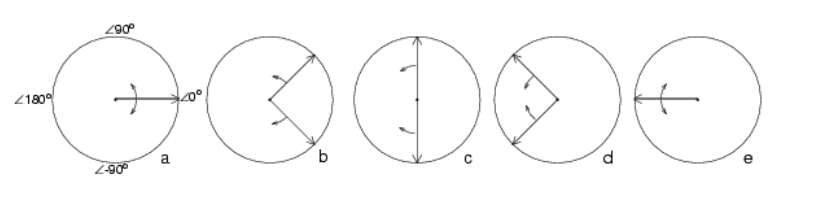
\includegraphics[width=0.8\textwidth]{assets/fasorenblauwenroodveld.png}
  \caption{Fasoren van de tegengestelde velden}
  \label{fig:fasorenblauwenroodveld.png}
 \end{figure}

Nu wat zijn we hiermee?
Dat we weten dat dit zo kan beschreven worden?
Awel, sinds dat dit 2 aparte fictieve draaivelden zijn kunnen die zich ook gedragen als
draaivelden van een gewone inductiemotor en genereren die dus elk een eigen
koppel-slip-curve die we in de volgende figuur met de stippenlijnen zien:

\begin{figure}[H]
  \centering
  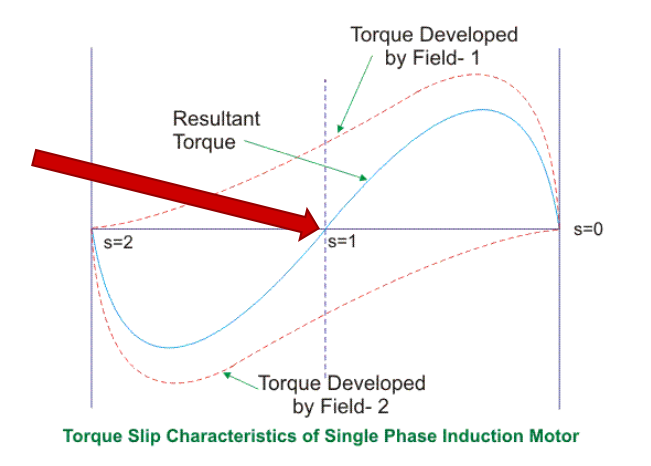
\includegraphics[width=0.8\textwidth]{assets/singlephadetorquetheoreticalapproach.png}
  \caption{1 fasige inductiemachine koppel theoretische benadering}
  \label{fig:singlephadetorquetheoreticalapproach.png}
 \end{figure}

De bovenste rode stippenlijn is dan voor dat rode draaiveld en de onderste rode stippelijn
is dan voor dat blauwe draaiveld (ik weet dat het confusing is dat beide stippelijnen rood
zijn en de vollelijn in het midden blauw $\#$shitfiguur).
Bij stilstand heeft de rotor exact dezelfde slip tegenover deze beide velden (ze draaien
evensnel in tegengestelde richting, dus evensnel tegengestelde koppels
$\rightarrow T_{res} = 0$).
Zodra de rotor een duwtje krijgt (bvb.
voorwaarts), wordt de slip tegenover het voorwaartse veld kleinen, dus veel koppel en de
slip van het achterwaartse veld groter, dus minder koppel.
Het netto koppel wordt dan positief (in de richting dat je hem duwde) en de motor
versnelt!

({\color{red}Volgende uitleg snap ik zelf niks van, AI kon het mij ook niet deftig
uitleggen, ik heb deze uitleg uit een samenvatting gevonden})
\newline
\textit{Een andere manier om deze werking te verklaren is een meer fysisch perspectief.
Voor de fysische betekenis van dit koppel gaan we kijken naar de figuur hier onder.
We hebben namelijk een rotor die ronddraait.
De stator heeft dan een wisselend magnetisch veld, waardoor in hetzelfde vlak een spanning
wordt geïnduceerd.
Dit is dus nog steeds hetzelfde als bij stilstand.
Maar omdat de rotor draait, en de rotor inductief is, gaat de stroom pas ontstaan als de
motor al gedraaid is.
Hierdoor gaan we dus ook een magnetisch veld opwekken in de rotor, wat staat volgens de
lijn van de maximale stroom.
Hierdoor gaat er dus ook een koppel ontstaan bij een motor.
}

\begin{figure}[H]
  \centering
  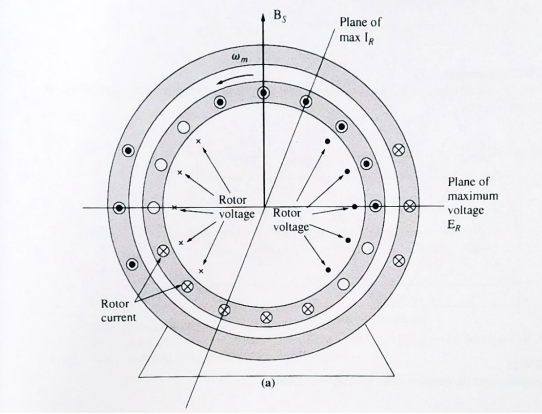
\includegraphics[width=0.4\textwidth]{assets/crossfieldtheory.png}
  \caption{Fysische betekenis (cross field theory)}
  \label{fig:crossfieldtheory.png}
 \end{figure}

(De uitleg die ik ervan heb verstaan in de les is dat als je op de rotor staat en deze in
beweging is (draait), dan zie je niet overal een even sterk veld want de stator is 1
wisselveld, dus ga je op sommige plaatsen in de rotor grotere stromen gaan hebben wat voor
een netto koppel zorgt (als de motor toch in bewegin is) en de motor gedraagt zich hier
dan inductief)

\subsection{Starten van een 1-fasige inductiemachine}
Nu gaan we dan kijken naar hoe we zo een 1-fasige machine kunnen starten aangezien ze geen
startkoppel hebben.
Hier zijn verschillende manieren voor, maar natuurlijk moet je ook in rekening houden dat
dit kleine machines zijn, dus ze aandrijven met een andere grote hulpmotor gaat niet
lukken (een kleine wel misschien).

Het makkelijkste dat we kunnen doen is hem natuurlijk manueel/extern aanduwen, gewoon een
klein duwtje geven en hij draait.
\textit{(Of zoals Prof.
Nobels het zei:
'We laten een chineesje de motor aanlopen!')}.
De andere manier om de motor te starten is met een \textbf{hulpwikkeling}, dit is een 2de
wikkeling die $90^\circ$ verschoven is tegenover die éne statorwikkeling zoals in volgende
figuur:

\begin{figure}[H]
  \centering
  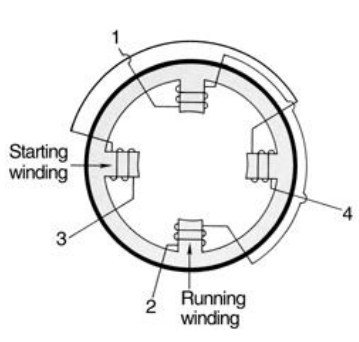
\includegraphics[width=0.4\textwidth]{assets/hulpwikkeling.png}
  \caption{Starting winding is die hulpwikkeling, de andere is de hoofdwikkeling}
  \label{fig:hulpwikkeling.png}
 \end{figure}

We doen dit want samen kunnen 2 wikkelingen wel een (bij benadering) draaiveld opwekken,
ideaal is dit dus natuurlijk een mooi rond draaiveld maar omdat beide wikkelingen hier op
dezelfde ééncontactspanning hangen (en we dus geen tweede fase eigelijk hebben) gaan we
deze hulpwikkeling elektrisch iets anders moeten bouwen dan de hoofdwikkeling (bvb.
dunnere draad, meer weerstand, minder inductief) zodat de stroom van nature een beetje
voorloopt tegenover de stroom in de (meer inductieve) hoofdwikkeling.
Zo hebben we wel een faseverschil en gaan we een draaiveld krijgen, dit draaiveld gaat
nooit exact $90^\circ$ zijn maar eerder een \textbf{elliptisch draaiveld} maar dit is nog
steeds sterk genoeg om de motor aan te lopen.
En hier is dan het speciale!
Eens dat de motor op snelheid is gekomen schakelt die \textbf{centrifugaal schakelaar} de
hulpwikkeling automatisch uit want die hulpwikkeling kan anders doorbranden en zowieso ook
voor te veel verliezen zorgen.
Wat we wel kunnen doen om dichter bij die $90^\circ$ te geraken is een condensator in
serie met de hulpwikkeling zetten, zo duw je eigelijk dat faseverschil dichter naar
$90^\circ$.
Hierdoor kan je een hoger opstartkoppel bereiken.
Dit noemt dan eigelijk de \textbf{condensator motor}, we kunnen deze ook tijdens het
normaal bedrijf van de motor verder laten draaien met nog een aparte kleinere condensator
wat net iets beter is of gewoon gebruiken enkel tijdens het opstarten en dan uitschakelen
met de centrifugaal en het verschil tussen de koppeltoerental karakteristiek van de deze
(met dus hulpwikkeling met condensator en de gewone motor met de hoofdwikkeling) ziet er
dan zo uit:

\begin{figure}[H]
  \centering
  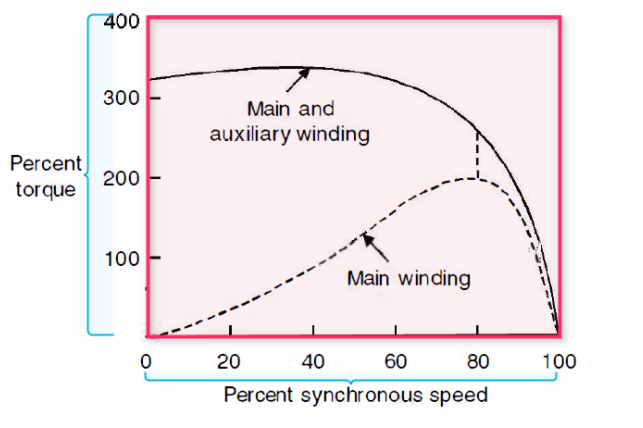
\includegraphics[width=0.5\textwidth]{assets/TNcondensatormotor.png}
  \caption{T-n karakteristiek van een condensator motor (met hulpwikkeling) vs gewone
  1-fasige inductiemotor}
  \label{fig:TNcondensatormotor.png}
 \end{figure}

De condensator motor wordt ook wel de beste 1-fasige motor genoemd.
De eer van de slechtste 1-fasige motor gaat naar de spleetpoolmotor.

\subsubsection{Spleetpoolmotor}
Dit is wel echt een heel kleine motor en heeft eigelijk meer als nut ook het starten van
de 1-fasige inductie-motor, het is dus niet echt een aparte variant van die motor, dit
dient vooral voor kleine vermogen met lage efficiënties.
Het is dus ook de goedkoopste/eenvoudigste manier om een 1-fasige inductiemotor te laten
starten (maar dus ook de slechtste).
Het idee is hier dat je geen aparte hulpwikkeling in deze kleine motor gebruikt maar dat
je met de hoofdwikkeling zelf hier 4 polen maakt en dat die polen eigelijk gesplitst zijn
fysiek.
Rond een deel van elk van die gesplitste polen wordt een kortgesloten koper ringetje
geplaatst (dus niet enkel op 1 pool, maar op elke pool, telkens aan dezelfde kant)
waardoor er daarin telkens een stroom wordt geïnduceerd door het feit dat de flux van de
hoofdwikkeling daar pulseert.
Wat dit doet is dan de verandering tegenwerking waardoor de flux in dat klein stukje
vertraagd wordt en er dus een soort van faseverschil ontstaat waardoor er een klein koppel
ontstaat.
Het statorveld wordt trouwens apart opgewekt en zo naar de rotor gebracht.
Je ziet dit in volgende figuur (die stator zijn de oranje wikkelingen, het veld wordt via
dat gelamelleerd ijzer verder gebracht):

\begin{figure}[H]
  \centering
  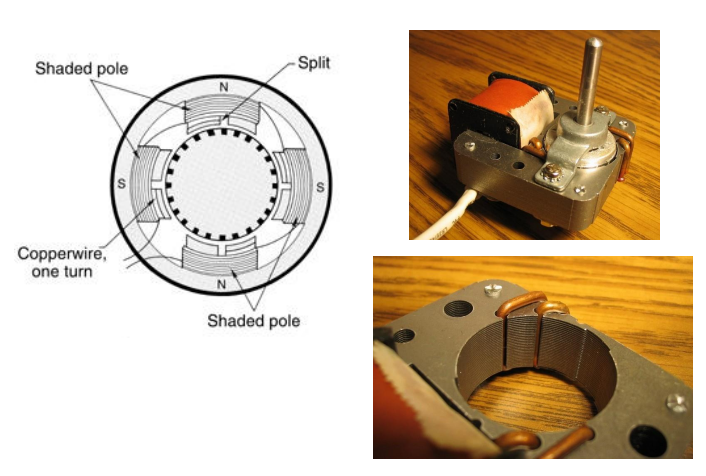
\includegraphics[width=0.6\textwidth]{assets/spleetpoolmotor.png}
  \caption{Spleetpoolmotor}
  \label{fig:spleetpoolmotor.png}
 \end{figure}

\subsection{Koppel-Toerental karakteristieken van de 1-fasige inductiemotoren}
De volgende grafiek toont alle besproken startmethodes naast elkaar van beste naar
slechtste koppel:

\begin{figure}[H]
  \centering
  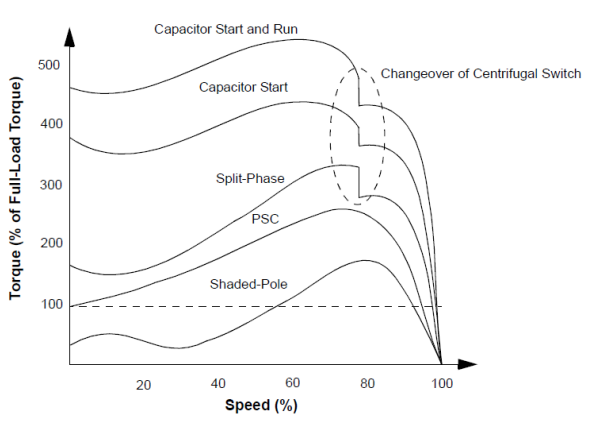
\includegraphics[width=0.6\textwidth]{assets/Tnkarakteritstieken1fmotore.png}
  \caption{Koppel-Toerental karakteristieken van de 1-fasige inductiemotoren}
  \label{fig:Tnkarakteritstieken1fmotore.png}
 \end{figure}

De 'Split-phase' motor is de gewone 1-fasige inductiemotor met hulpwikkeling trouwens, de
PSC (Permanent Split Capacitor) is condensator + hulpwikkeling zonder een schakelaar,
capacitator start en run heeft een kleine runcondensator nog en capacitator start is
gewoon de grotere normale condensator helemaal los (had nooit zo een run condensator) en
shaded pole is dus de spleetpoolmotor, je ziet dat deze ook gekke effecten heeft en dus
een slecht rendement.

En in volgende tabel zien we nog rap een kort overzicht van de 5 verschillende 1-fasige
motors:

\begin{figure}[H]
  \centering
  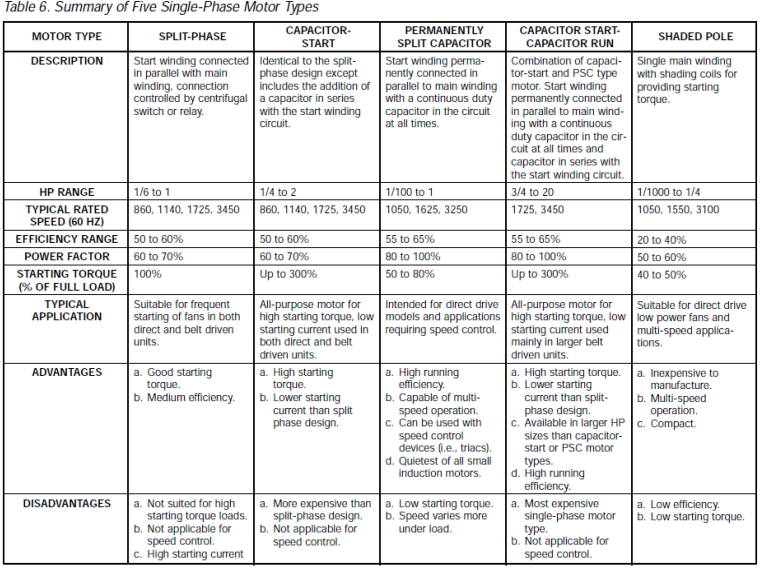
\includegraphics[width=0.6\textwidth]{assets/tabel1fmotors.png}
  \caption{Tabel van de 5 verschillende 1-fasige inductiemotoren}
  \label{fig:tabel1fmotors.png}
 \end{figure}

We zien dat de 'permanently split capacitator' en 'capacitator start capacitator run'
motoren het beste rendement hebben.

\section{BLDC (Brushless DC) motor}
Dan gaan we nu over naar de vermogenelektronica gestuurde motoren, we gaan eigelijk vooral
de deze bespreken.
De BLDC is elektrisch gezien een DC machine maar dan \textit{zonder een mechanische
commutator en borstels}.
Wat hier ook belangrijk is, is dat\textbf{ het anker hier de stator is en de bekrachtiging
de rotor!} Dit was omgekeerd bij de normale DC-machine!!!
De wikkelingen zitten bij de BLDC dus vast op de stator en draaien de permanente magneten
mee met de rotor (zelfde opbouw als de permanentmagneet synchroonmachine).
Doordat er geen borstels zijn \textit{kan de BLDC niet rechtstreeks op een batterij (of
stopcontact) aangesloten worden}, we hebben hier dus altijd een elektronische controller
nodig die de stroom naar de juiste wikkeling op het juiste moment stuurt.
Hier is voor de zekerheid en verduidelijk nog een tabel waarin staat wat het anker en wat
de bekrachtiging is bij de (PM)DC, BLDC en (PM)SM:

\begin{figure}[H]
  \centering
  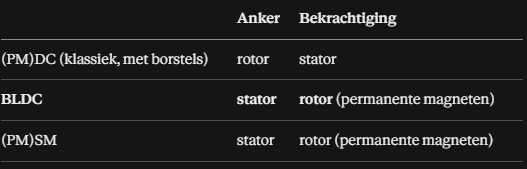
\includegraphics[width=0.6\textwidth]{assets/tabelmachinesankerbekrachtiging.png}
  \caption{Tabel van de anker- en bekrachtigingswikkelingen van de verschillende machines}
  \label{fig:tabelmachinesankerbekrachtiging.png}
 \end{figure}

\subsection{Werking van de BLDC motor}
Dus bij de BLDC heb je niet de commutator met borstels dat als mechanische inverter werkt
en ervoor zorgt dat de stroom door de rotors steeds in de juiste richting staat, hier ga
je het dus moeten doen met elektronica.
Om te weten wanneer er precies moet geschakeld worden moet de controller dus weten waar de
rotor zich precies bevindt.
Dit gebeurt met \textbf{Hall-sensoren}, door er zo 3 te gebruiken en dit een simpel
digitaal signaal te doen genereren afhankelijk van welke pool er voorbij komt kan met een
paar berekeningen de exacte sector (1 van de 6 in de figuren die ik ga tonen) bepaald
worden van 1 omwenteling.
De controller zelf die weet precies via deze hall waardes welke stroom gestuurd moet
worden (-10, 0 of 10 A, 10 is gewoon een voorbeeld van een DC stroom).
Via transistoren worden die stromen dan geschakeld.
Bij elke overgang naar zo een nieuwe sector schakelt de controller de volgende combinatie
van transistoren, dit heet \textbf{6-staps-(of trapezoïdale) commutatie}.

\begin{figure}[H]
  \centering
  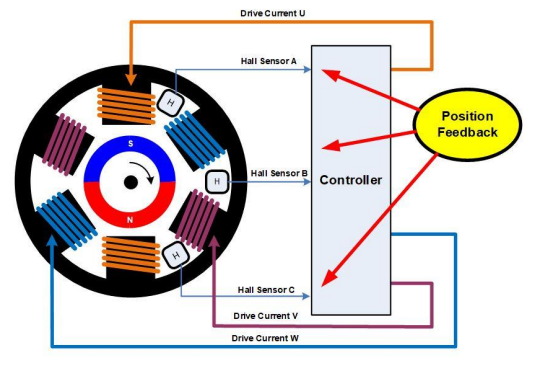
\includegraphics[width=0.5\textwidth]{assets/hallsensorsmetcontroller.png}
  \caption{BLDC met hall sensor en controller}
  \label{fig:hallsensorsmetcontroller.png}
 \end{figure}

\begin{figure}[H]
  \centering
  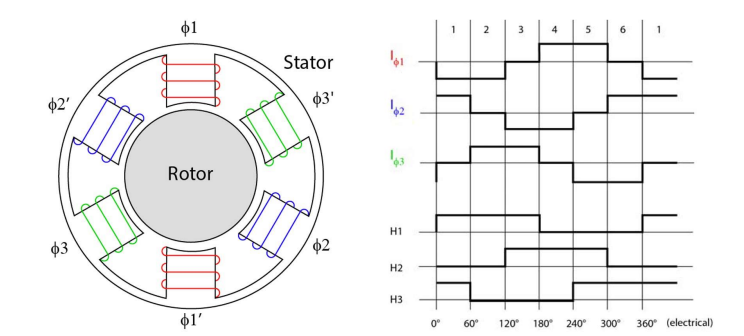
\includegraphics[width=0.6\textwidth]{assets/hallsensorgestuurdestromen.png}
  \caption{Stromen gestuurd door de hall sensor}
  \label{fig:hallsensorgestuurdestromen.png}
 \end{figure}

\begin{figure}[H]
  \centering
  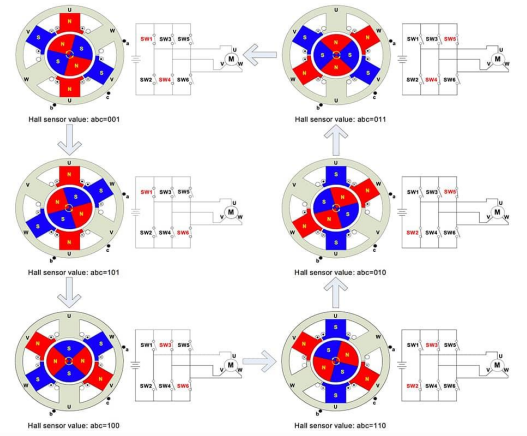
\includegraphics[width=0.6\textwidth]{assets/6stapscommutatie.png}
  \caption{6-staps commutatie}
  \label{fig:6stapscommutatie.png}
 \end{figure}

\subsection{Terug-emk (back-emf) van de BLDC motor}
Terwijl dat de rotor draait (met zijn magneten dus) zien de statorspoelen dus ook een
veranderd magnetisch veld voorbij komen wat dus een spanning induceert in de spoel
($e = B \cdot l \cdot v$).
Dit is het terug-emk en deze wordt groter naarmate de rotor sneller draait (zoals bij alle
DC en AC machines).
Wat er echter speciaal is, is dat deze een \textbf{trapezoïdale vorm} heeft i.p.v.
een mooie sinus, zoals we kunnen zien in volgende figuur:

\begin{figure}[H]
  \centering
  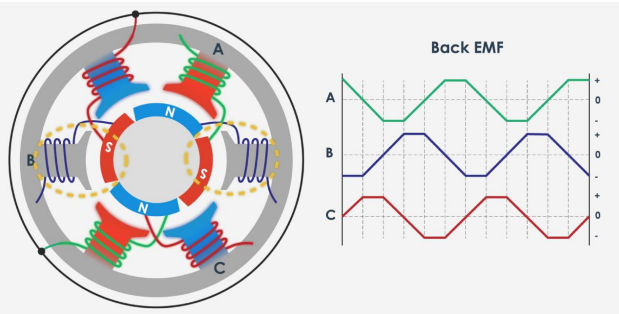
\includegraphics[width=0.6\textwidth]{assets/tegenemkbldc.png}
  \caption{Terug-emk van de BLDC motor}
  \label{fig:tegenemkbldc.png}
 \end{figure}

Dit komt doordat als een spoel volledig onder zo één magneetpool zit, ze eigelijk ongeveer
een constant veld ziet steeds, dit maakt het constant in die emf-curve, pas wanneer de
rotor verder draait en de zuidpool wegschuift terwijl de volgende noordpool binnekomt
veranderd het veld snel van volledig negatief naar volledig positief wat dus die schuine
flank geeft (uiteindelijk trapezium dus).
Het feit dat dit wel een mooie sinus is bij de PMSM terwijl die ook permanente magenten
gebruikt is door het feit dat daar de statorwikkelingen verdeeld zijn in plaats van
geconcentreerd rond de polen zoals hier.

\begin{figure}[H]
  \centering
  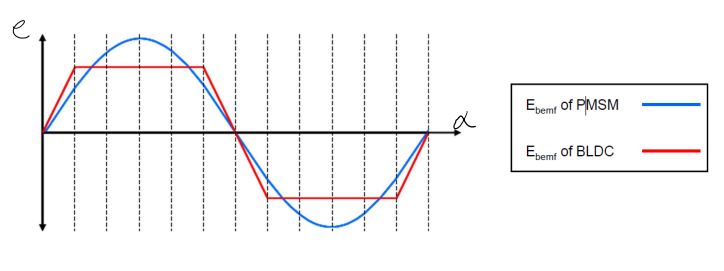
\includegraphics[width=0.7\textwidth]{assets/tegenemkbldcpmsm.png}
  \caption{Terug-emk van de BLDC en de PMSM motor}
  \label{fig:tegenemkbldcpmsm.png}
 \end{figure}

Nog iets belangrijk om te onthouden bij deze 2 motoren is dat doordat we permanente
magneten gebruiken er geen vermogenverlies nodig is om het rotor veld zelf op te wekken.

\subsection{Koppel-toerental karakteristiek van de BLDC motor}
Net zoals de DC-machine heeft een BLDC motor een continue koppelzone (het groene) en ook
een korstondige/intermittente zone (geel/snotgroen) erboven:

\begin{figure}[H]
  \centering
  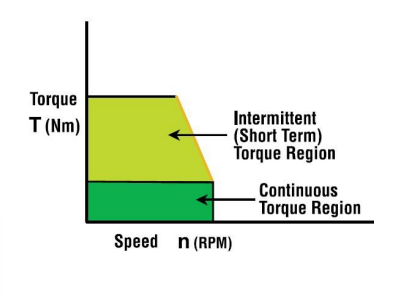
\includegraphics[width=0.5\textwidth]{assets/TNBLDC.png}
  \caption{Koppel-toerental karakteristiek van de BLDC motor}
  \label{fig:TNBLDC.png}
 \end{figure}

Er is ook een T-limiet (het plafond), dit is bepaald door de maximale stroom die door de
wikkelingen continu kan gaan zonder oververhitting.
In de gele zone kan je kort even werken met meer stroom/koppel.
Ook is er een n-limiet, dit is eigelijk een begrenzing door mechanische factoren zoals de
constructie van de rotor of lagers of door de schakel/commutatie elektronica zelf (de
transistoren kunnen tot maar een bepaalde frequentie schakelen).

De volgende grafiek toont de verschillende lijnen voor verschillende spanningen, hoe hoger
de spanning, hoe hoger de bereikbare snelheid bij een gegeven koppel.
(Dit zagen we eerder bij de DC machine), het belangrijkste hier is omdat een BLDC via
vermogenelektronica aangestuurd wordt, je niet gelimiteerd bent tot 1 van die lijnen, de
controller kan elke spanning tot aan $V_1$ leveren.
Dus eigelijk kan je in de praktijk eender welk werkingspunt in het oppervlak onder de
$V_1$ lijn aannemen.

\begin{figure}[H]
  \centering
  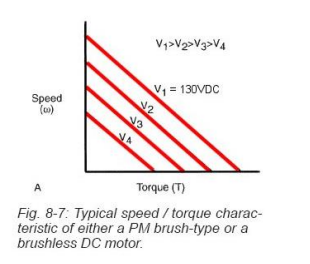
\includegraphics[width=0.5\textwidth]{assets/VlijnenBLDC.png}
  \caption{Spanningslijnen van de BLDC motor}
  \label{fig:VlijnenBLDC.png}
 \end{figure}

\subsection{BLDC vs (PM)Borstel DC motor}
Nu gaan we enkele voor- en nadelen vergelijken van de BLDC met de gewone (PM)DC motor.
\newline
\textbf{{\color{green}Voordelen} van de BLDC:}

\begin{itemize}
    \item Langere levensduur (geen borstels/commutator die slijten)
    \item Minder geluid en elektrische storing (geen vonken van de borstels)
    \item Makkelijker te koelen:
    Bij een BLDC zitten alle koperverliezen in de wikkelingen op de stator, die staat stil
    en is dus makkelijk te koelen, bij een PMDC zit het anker juist op de rotor, warmte
    afvoeren van een ronddraaiend deel is lastiger
    \item Beter rendement dankzij elektronische sturing
\end{itemize}

\textbf{{\color{red}Nadelen} van de BLDC:}

\begin{itemize}
 \item Hogere kost
 \item Trillingen bij lage snelheid (door de 6-staps commutatie)
 \item Complexe elektronica nodig (controller, hall sensoren, $\cdots$)
\end{itemize}

Een samenvattende figuur van voor en nadelen voor ook de inductiemotor en stappenmotor
zien we in volgende figuur:

\begin{figure}[H]
  \centering
  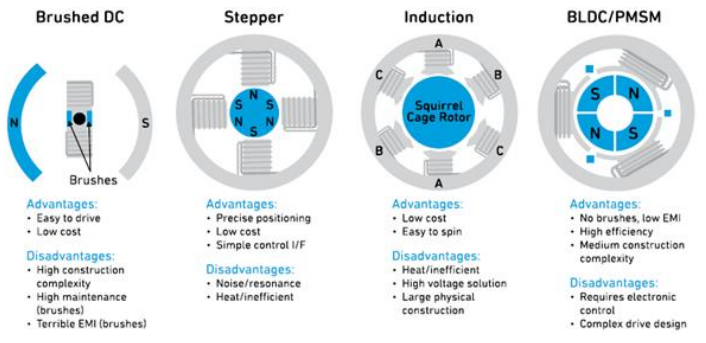
\includegraphics[width=0.8\textwidth]{assets/vergelijkingenmotore.png}
  \caption{Vergelijking van de verschillende motoren}
  \label{fig:vergelijkingenmotore.png}
 \end{figure}

\section{Reluctantie motoren}
Een reluctantie motor is een nieuw type motor, het positioneert zich als een concurrent
van de inductiemachine.
Het is een soort synchrone motor.
Het bijzondere aan deze motor is dat \textit{de rotor enkel bestaat uit ijzer}, dus geen
wikkelingen of magneten of kooi ofzo.
Dit maakt het super goedkoop en robuust (geen koperverliezen op de rotor, geen dure
magneten en praktisch INDESTRUCTABLE).
Maar hoe werkt het?

\begin{figure}[H]
  \centering
  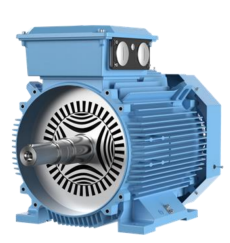
\includegraphics[width=0.4\textwidth]{assets/fotoreluctantiemotor.png}
  \caption{Reluctantie motor}
  \label{fig:fotoreluctantiemotor.png}
 \end{figure}

\subsection{Werking van de reluctantie motor}
We zagen dit concept al eerder maar deze motor werkt hier dus volledig op, namelijk het
\textbf{reluctantiekoppel}.
Reluctantie is de magnetische weerstand eigelijk, het is hoe makkelijk de flux door een
pad kan vloeien en ijzer heeft een veel lagere reluctantie dan lucht.
Het kernprincipe van deze motor is dat elk magnetisch systeem probeert zijn energie te
minimaliseren, dus door zijn reluctantie te minimaliseren.
Een stuk ijzer dat scheef staat tegenover een veld 'voelt' daardoor een koppel dat het
terug wilt uitlijnen met dat veld (want het is het pad van minst reluctantie).
Dit zien we in de volgende figuur:

\begin{figure}[H]
  \centering
  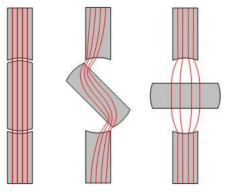
\includegraphics[width=0.4\textwidth]{assets/padvanminstreluctantie.png}
  \caption{Pad van minst reluctantie}
  \label{fig:padvanminstreluctantie.png}
 \end{figure}

In de volgende figuur zien we hoe dit toegepast wordt met de stator en de rotor, hoe meer
overlap tussen de stator en rotortanden, hoe lager de reluctantie:

\begin{figure}[H]
  \centering
  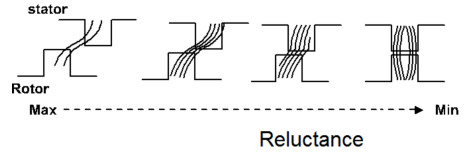
\includegraphics[width=0.8\textwidth]{assets/sgtatorrotorreluctantie.png}
  \caption{Overlap tussen stator en rotor}
  \label{fig:sgtatorrotorreluctantie.png}
 \end{figure}

Er zijn 2 varianten van reluctantiemotoren, we hebben de \textbf{synchrone reluctantie
motor} en de \textbf{'switched' reluctantie motor} (SRM).

\begin{figure}[H]
  \centering
  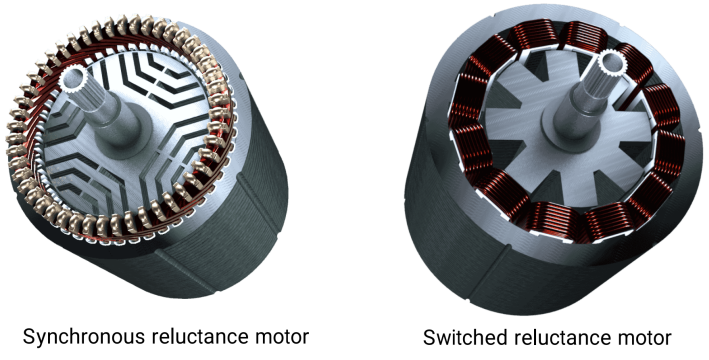
\includegraphics[width=0.6\textwidth]{assets/synchroneenswitchedreluctantiemotor.png}
  \caption{Varianten van reluctantiemotoren}
  \label{fig:synchroneenswitchedreluctantiemotor.png}
 \end{figure}

De \textbf{synchrone reluctantiemotor} heeft een rotor met interne 'flux barrieres' die
voorkeursrichtingen voor de flux creëren, het wordt aangedreven door een gewoon draaiveld
zoals bij de inductiemotor en loopt daarmee synchroon mee (geen slip)

De \textbf{'switched' reluctantiemotor} heeft een getande rotor en stator en wordt
aangedreven door telkens een paar statorspoelen gericht aan en uit te schakelen (daarom
'switched'), dit is hoe steeds de dichtsbijzijnde rotortand telkens zo wilt uitlijnen met
een bekrachtigde statortand zoals in die figuur die ik net toonde.
Dit is een beetje gelijkaardig aan de BLDC, daar was het aantrekken met een magneet.

\subsection{Nadelen van de 'switched' reluctantiemotor}
De 'switched' reluctantiemotor heeft echter een paar nadelen, namelijk dat we een
koppelrimpel hebben doordaat we steeds gaan uitlijnen met die tanden en dit zorgt voor
\textbf{trillingen}.
ook heeft het een \textbf{ingewikkelde constructie/sturing}, die dubbel getande geometrie
is lastig te ontwerpen en verreist ook nauwkeurige sturing.
ook is er veel \textbf{ijzerverzadiging} rond de uitgelijnde tanden wat het stroom-koppel
verband minder lineair maakt en dus de sturing bemoeilijkt.

\subsection{Werking van de synchrone reluctantiemotor}
Het is dus de deze dat dan meer gebruikt wordt als we het gaan hebben over de reluctantie
motor.
De rotor is  hier opgebouwd uit gelamelleerd ijzer met halfronde luchtspleten (flux
barrieres) die in lagen boven elkaar zitten, dit zie je in de figuur hieronder links.
Dit maakt de opbouw eigelijk anisotroop, in de ene richting geleidt hij flux makkelijk
(rood) en in de andere richting bijna niet (blauw).

\begin{figure}[H]
  \centering
  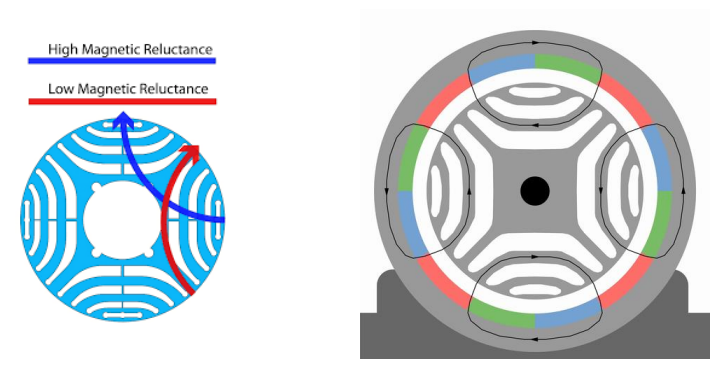
\includegraphics[width=0.6\textwidth]{assets/synchronereluctantiemotor.png}
  \caption{Synchrone reluctantiemotor}
  \label{fig:synchronereluctantiemotor.png}
 \end{figure}

Op het rechtse gedeelte van de figuur zien we blauwe/groene/rode zones, dit representeert
de 3fases van de statorwikkelingen, er wordt een draaiveld opgewekt en net zoals bij de
inductiemotor gaat de rotor voelen dat het niet perfect samen uitgelijnd is met het
draaiveld en zich proberen uitlijnen dan.
Omdat het veld blijft roteren blijft dit gebeuren en gaat de rotor dus mooi synchroon
meedraaien met dat veld (geen slip).
Ook omdat de rotor bij synchroon, continu draaien geen relatieve fluxverandering
ondervindt zijn de ijzerverliezen in de rotor (tijdens continu bedrijf) minimaal, dit
geeft deze motor een hoog rendement voor dit motortype toch.
Geen rotorkoperverliezen hier en amper ijzerverliezen.
Alleen bij transiënten (opstarten en belastinswissels) kunnen we wat verliezen hebben
omdat de flux dan nog aan het 'instellen' is.

\section{Stappen motoren}
Dit moeten we niet uitgebreid meer kennen, dit is een volledig ander concept.
We moeten vooral weten dat dit een positiegestuurde motor is en dat dit in plaats van een
T-n karakteristiek een 'aantal stappen per omwenteling' heeft.
Het werkt met 'open loop position control' (Elke puls die je stuurt doet de rotor exact
één vaste, discrete hoek verspringen).

{\color{red}Alle slides/leerstof hier na moeten we niet meer kennen, dit is het einde van
de leerstof}
